\documentclass[10pt]{article}
\usepackage[utf8]{inputenc}
\usepackage{float}
\usepackage{url}
\usepackage[portuguese]{babel}
\usepackage{graphicx}
\usepackage{microtype}
\usepackage[T1]{fontenc}

\title{IF755 - REALIDADE VIRTUAL}
\author{Jonathas vinicius }
\date{\vspace{-5ex}}

\usepackage{natbib}

\begin{document}

\maketitle

\section{Introdução}

A disciplina de realidade virtual tem como objetivo fazer com que os discentes aprendam a programar com algumas linguagens especificas para esta areá, nela também se aprende conceitos avançados e ferramentas para VR/AR desenvolvendo a capacidade do aluno para construir tecnologias que suportem o desenvolvimento de VR/AR e seus sistemas tendo aplicações em áreas como jogos,marketing e medicina.

\begin{itemize}
  \item seus objetivos são fazer com que o discente Conheça conceitos avançados e ferramentas para
- Realidade Virtual (VR)
- Realidade Aumentada (AR)
- Desenvolver a capacidade de
- Construir tecnologia que suporte o desenvolvimento de VR e / ou AR
sistemas
- Construir soluções inovadoras de RV e / ou AR, focando diversas
domínios de problema .\cite{primeira}
\end{itemize}

A disciplina está inserida na área de MÍDIAS E INTERFACES , sendo o seu profissional é responsável pelo desenvolvimento e criação de programas e sistemas de realidade virtual ou aumentada (VR/AR).

\begin{figure}[]
    \centering
    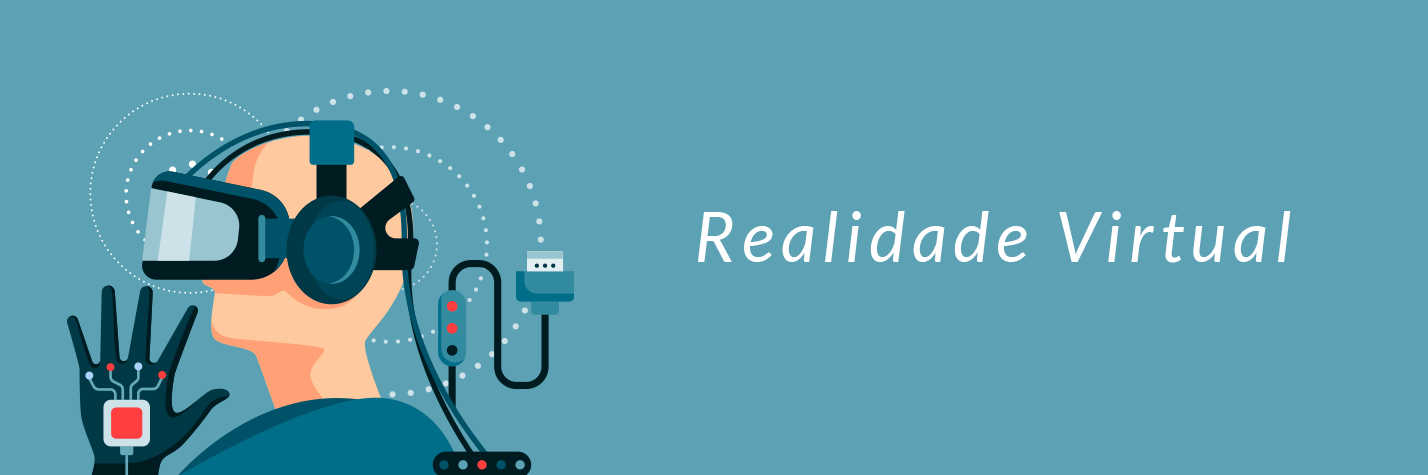
\includegraphics[scale=0.15]{realidadevirtual.png}
    \caption{REALIDADE VIRTUAL \cite{quinta}}
    \label{fig:realidadevirtual}
\end{figure}

\section{Relevância}
essa cadeira e voltada para pessoas com interesses em computação gráfica, processamento de imagens ou visão computacional.sendo uma inovação e natural que cientistas da computação queiram no currículo por abrir portas para o mundo da tecnologia e do trabalho.\cite{segunda}

\section{Relações}


algumas disciplinas que são relacionadas com a realidade virtual que estão na grade curricular e o motivo de estarem relacionada
\begin{center}
\begin{tabular}{|c|p{10cm}|}
\hline
códigos & relações \\ \hline
 IF681 Interface Usuário Maquina &
 Nesta disciplina são demonstrados conceitos ainda básicos de design de interação e design thinking para a concepção de sistemas computacionais interativos.\cite{terceira}
 \\ \hline
 IF687 Introdução à Multimídia  & 
Basicamente e o primeiro contato com o mundo virtual e de aplicações de multimídia vem desta disciplina seus objetivos são desenvolver a capacidade de propor e criar e avaliar mundos virtuais ênfase na internet, visando aplicações em medicina por exemplo
Desenvolver também a capacidade de especificar, construir e avaliar componentes multimídia específicos para esse mundo. \cite{quarta} \\ \hline

\end{tabular}    
\end{center}


\bibliographystyle{plain}
\bibliography{jvras}

\end{document}